%%%%%%%%%%%%%%%%%%%%%
%% Desenvolvimento %%
%%%%%%%%%%%%%%%%%%%%%

\section{Introdução}

A partir deste ponto, o ambiente de trabalho está pronto para ser utilizado. Neste capítulo, são apresentados detalhes do processo de desenvolvimento, e nos próximos, detalhes sobre funcionalidades específicas do sistema e fragmentos de código, tornando facilmente adquirível o conhecimento necessário para fazer alterações, aprimoramentos e correções na aplicação. 

%%%%%%%%%%%%%%%%%%%%%

\section{Repositório}

\subsection{Organização do Repositório}
O SAEC é dividido em 4 repositórios diferentes:
    \begin{itemize}
        \item \textbf{code}: código da aplicação;
        \item \textbf{phplibcryptosec}: código do wrapper PHP5LibCryptoSec;
        \item \textbf{makepkg}: script para a geração do pacote de instalação da aplicação;
        \item \textbf{doc}: documentação do projeto.
    \end{itemize}

\vspace{5mm}

O repositório principal, \textit{code}, está dividido em diversas branches:
    \begin{itemize}
        \item \textbf{master}: é atualizado quando uma nova versão é lançada;
        \item \textbf{dev}: é o mais utilizado durante o desenvolvimento;
        \item \textbf{release}: utilizado para maturação de uma nova versão;
        \item \textbf{SAEC-X}: utilizados para a realização de tarefas.
    \end{itemize}

\begin{figure}[h]
  \begin{center}
    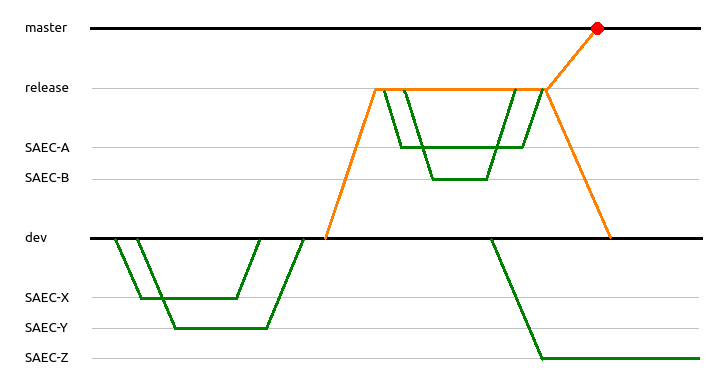
\includegraphics[scale=0.58]{images/git.png}
    \caption{Fluxo do Repositório}
    \label{fig:fluxobranches}
  \end{center}
\end{figure}

\vspace{5mm}

O fluxo do repositório, representado pela figura \ref{fig:fluxobranches}, funciona da seguinte maneira: Para cada tarefa de desenvolvimento é criado um novo branch temporário com o nome \textbf{SAEC-X}, onde X é um número que identifica a tarefa. Quando a tarefa é concluída, deve ser aberto um \textit{merge request} para o branch \textbf{dev}. Quando julgar-se necessário o lançamento de uma nova versão do software com as alterações contidas no \textbf{dev}, é feito um \textit{merge} dele para o branch \textbf{release} e é lançada uma nova versão para testes, com o código contido neste branch. Após realizados os testes e as correções necessárias, são feitos \textit{merges} do branch \textbf{release} para o \textbf{dev} (para incluir nele as correções feitas) e \textbf{master}, onde é criada uma \textit{tag} para a nova versão.

\subsection{Usando o Git}

Para começar o desenvolvimento de uma tarefa, deve-se primeiro verificar se o branch local é o \textit{dev}. Para isso, no diretório onde está o código, o comando \textit{branch} pode ser executado. Caso não seja, basta realizar um \textit{checkout}.

\begin{lstlisting}[language=bash]
    $ git branch
    $ git checkout dev
\end{lstlisting}

Estando no branch \textit{dev}, deve-se realizar um \textit{pull} do repositório para atualizar o código local e criar um novo branch \textit{SAEC-X}, onde X é o número que identifica a tarefa que será realizada.

\begin{lstlisting}[language=bash]
    $ git pull origin dev
    $ git checkout -b SAEC-X
\end{lstlisting}

Terminado o desenvolvimento, podem ser utilizados os comandos \textit{status} e \textit{diff} para visualizar as alterações feitas. Caso seja necessário reverter as alterações em algum arquivo, basta utilizar o comando:

\begin{lstlisting}[language=bash]
    $ git checkout -- <caminho_do_arquivo>
\end{lstlisting}

Após verificar que as alterações feitas estão corretas, pode ser feito o commit.

\begin{lstlisting}[language=bash]
    $ git add -A
    $ git commit -m "SAEC-X: Mensagem descrevendo o que foi feito"
    $ git push origin SAEC-X
\end{lstlisting}

Feito o commit, deve-se então entrar no GitLab e criar um \textit{merge request}, para que seu código seja revisado e incluído na branch \textit{dev}.